\documentclass[fleqn, 10pt]{article}


\usepackage[utf8]{inputenc}
\usepackage{amsthm, amsmath}
\usepackage{nccmath} %Para centrar ecuaciones
\usepackage{graphicx}
\usepackage{enumitem}
\usepackage{whilecode2}

\graphicspath{ {} } 

    \title{\textbf{Practica 3}}
    \author{Daniel García Villodres}
    \date{}
    
    \addtolength{\topmargin}{-3cm}
    \addtolength{\textheight}{3cm}
    

    
\begin{document}

\maketitle
\thispagestyle{empty}

\section*{Actividad 1}
Define the TM solution of exercise 3.4 of the problem list and test its correct
behaviour.


\subsection*{}
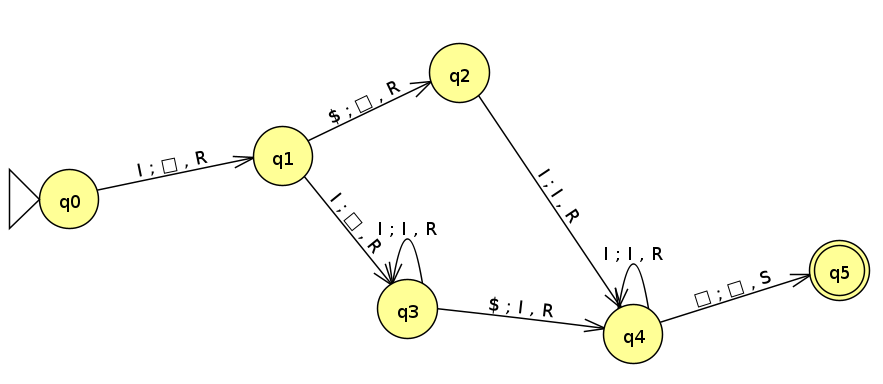
\includegraphics[scale=0.5]{MT}


\section*{Actividad 2}
Define a recursive function for the sum of three values.

\subsection*{}

$<<\pi^1_1|\sigma\left(\pi^3_3\right)>|\sigma\left(\pi^4_4\right)>$

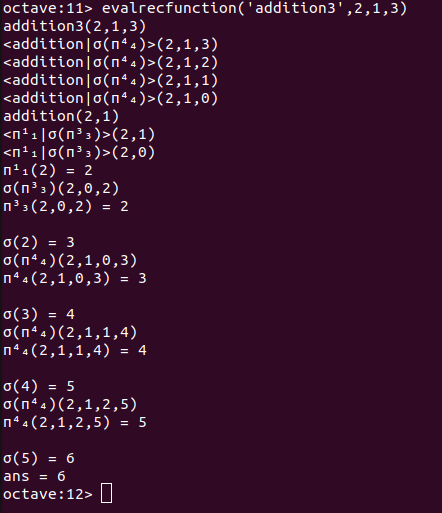
\includegraphics[scale=0.5]{FuncionR.png}


\section*{Actividad 3}
Implement a WHILE program that computes the sum of three values. You
must use an auxiliary variable that accumulates the result of the sum.

\subsection*{}
\whileprogram{Q}{3}{
\begin{whilecode}[H]

 \While{$G(X_1) \not = 0$}{

  $X_1 \Assig X_1 - 1$\;
  $X_4 \Assig X_4 + 1$\;
  
 }
 \While{$G(X_2) \not = 0$}{

  $X_2 \Assig X_2 - 1$\;
  $X_4 \Assig X_4 + 1$\;
  
 }
 \While{$G(X_3) \not = 0$}{

  $X_3 \Assig X_3 - 1$\;
  $X_4 \Assig X_4 + 1$\;
  
 }
  $X_1 \Assig X_4$\;
\end{whilecode}
}{s}



\end{document}
